\documentclass[compress, color = usenames, dvipsnames]{beamer}

% theme CentraleSupelec
\usepackage{theme/beamerthemeCS}

% liste de paquets
\usepackage[utf8]{inputenc}
\usepackage[francais]{babel}
\usepackage{xstring}
\usepackage{tikz}
\usetikzlibrary{shapes.arrows,chains,fit, calc,positioning, intersections}
\usepackage{pgfplots}
\usepackage{hyperref}
\usepackage{listings}
\usepackage{verbatim}
\usepackage{hyperref}
\usepackage{multimedia}
\usepackage{ifthen}

\usepackage{xcolor}% http://ctan.org/pkg/xcolor
\usepackage{colortbl}

\usepackage{pifont}
\usepackage{textcomp}
\usepackage{textpos}

\usepackage{soul}
%\usepackage{algorithmic}
\usepackage{algpseudocode}



% première page
\title[Jeu de Go \\ et \\ Exploration d'Arbre par Bandit]{Jeu de Go \\ et \\ Exploration d'Arbre par Bandit}
\subtitle[]{}
\date[]{}
\institute[]{\large CentraleSupélec -- Gif}


\begin{document}

\frame{
  \titlepage
}

\frame{
  \frametitle{IA et Jeu de Go}

  \begin{center}
  \includegraphics[width=0.8\textwidth]{figs/badukia.jpg}
  \end{center}

  \begin{itemize}
      \item 2016: AlphaGo bat le meilleur joueur humain 
      \item Combine des méthodes de \textbf{deep learning} avec une \red{exploration d'arbre par bandit}
  \end{itemize}

}




\section{IA et Jeu de Go}


\subsection{Pourquoi une IA pour le Jeu de Go?}

\frame{
  \frametitle{Pourquoi une IA pour un jeu?}

  \begin{center}
  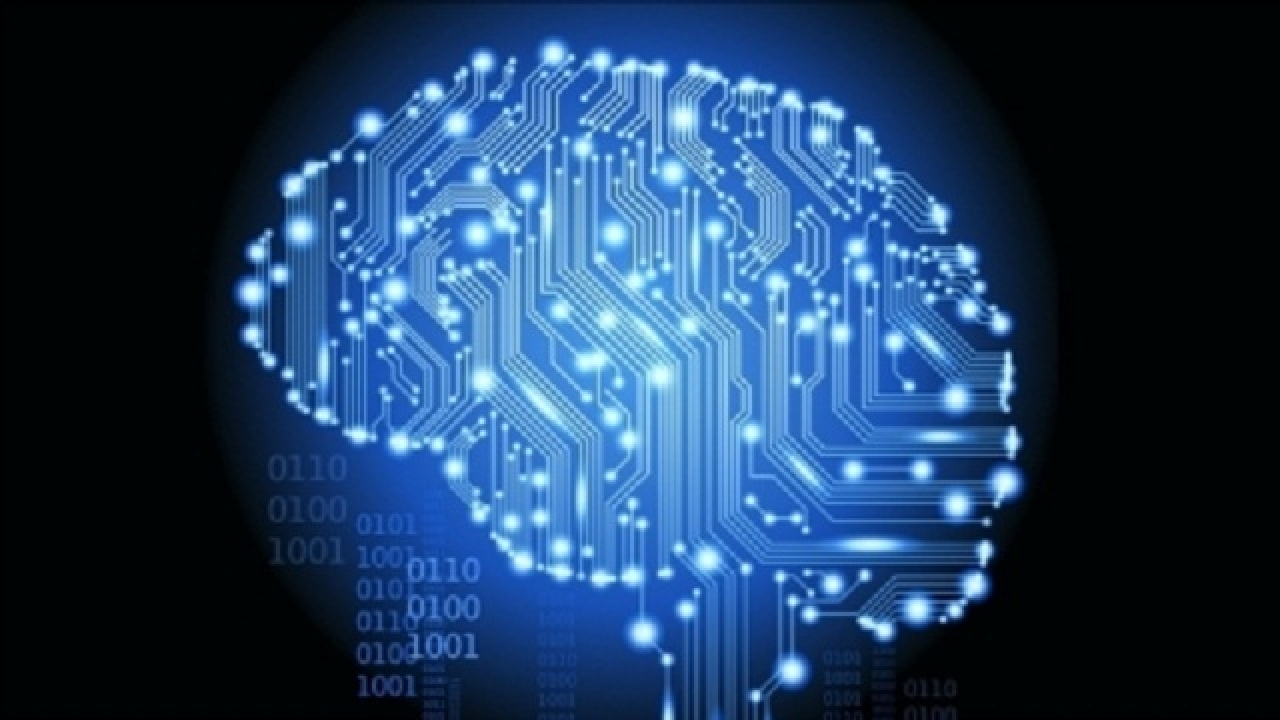
\includegraphics[width=0.5\textwidth]{figs/aigame.jpg}
  \end{center}
  \begin{itemize}
      \item Avoir une IA pour un jeu...
      \item Représentation des \red{problèmes de décision}
      \item \textbf{Environnement} bien défini: règles du jeu
      \item \textbf{Évaluation} facile: score
      \item \red{Challenge} de battre les humains
  \end{itemize}


}

\frame{
  \frametitle{Pourquoi le jeu de Go?}

  \begin{center}
  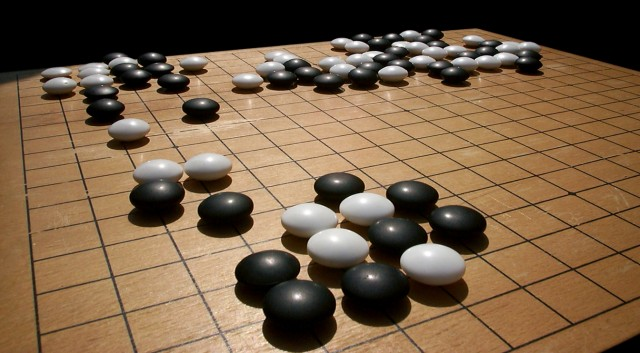
\includegraphics[width=0.5\textwidth]{figs/go-intro.jpg}
  \end{center}

  \begin{itemize}
      \item un jeu de plateau qui a longtemps résisté aux IA
      \item règles \textbf{simples}
      \item méthodes classiques (alphabeta) inefficaces
  \end{itemize}

}


\subsection{Le Jeu de Go}

\frame{
  \frametitle{Histoire}

  \begin{columns}
      \begin{column}{0.3\textwidth}
          \begin{center}
              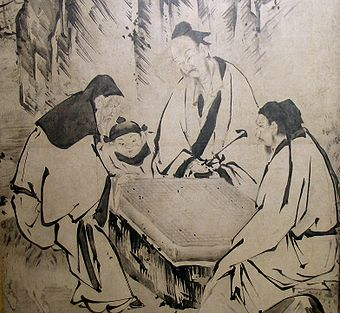
\includegraphics[width=1\textwidth]{figs/gohistory.jpg}
          \end{center}
      \end{column}
      \begin{column}{0.7\textwidth} 
          \begin{itemize}
              \item aurait été inventé en chine en 2000 BC
              \item premiers écrits: 500 BC
              \item fait parti des 4 arts majeurs chinois: peinture, calligraphie, guqin, \textit{go}
              \item se répand en Asie dès 800 dans la noblesse
              \item aujourd'hui, environ 20 millions de joueurs
          \end{itemize}
      \end{column}
  \end{columns}


}

\frame{
  \frametitle{Matériel}

  \begin{columns}
      \begin{column}{0.6\textwidth}
          \begin{itemize}
              \item plateau de jeu: Goban
              \item deux tailles 9x9 ou 19x19
              \item pierres noires et blanches 
          \end{itemize}
      \end{column}
      \begin{column}{0.4\textwidth} 
          \begin{center}
              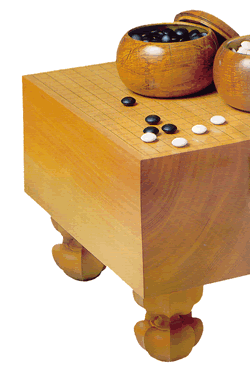
\includegraphics[width=1\textwidth]{figs/gomatos.png}
          \end{center}
      \end{column}
  \end{columns}



}

\frame{
  \frametitle{Règles: placement}

  \begin{itemize}
    \item Début de la partie: le plateau est vide
    \item Chaque joueur pose une pierre à tour de rôle
    \item Noir commence
    \item Pierres posées sur les intersections
  \end{itemize}

  \begin{center}
      \only<1> { 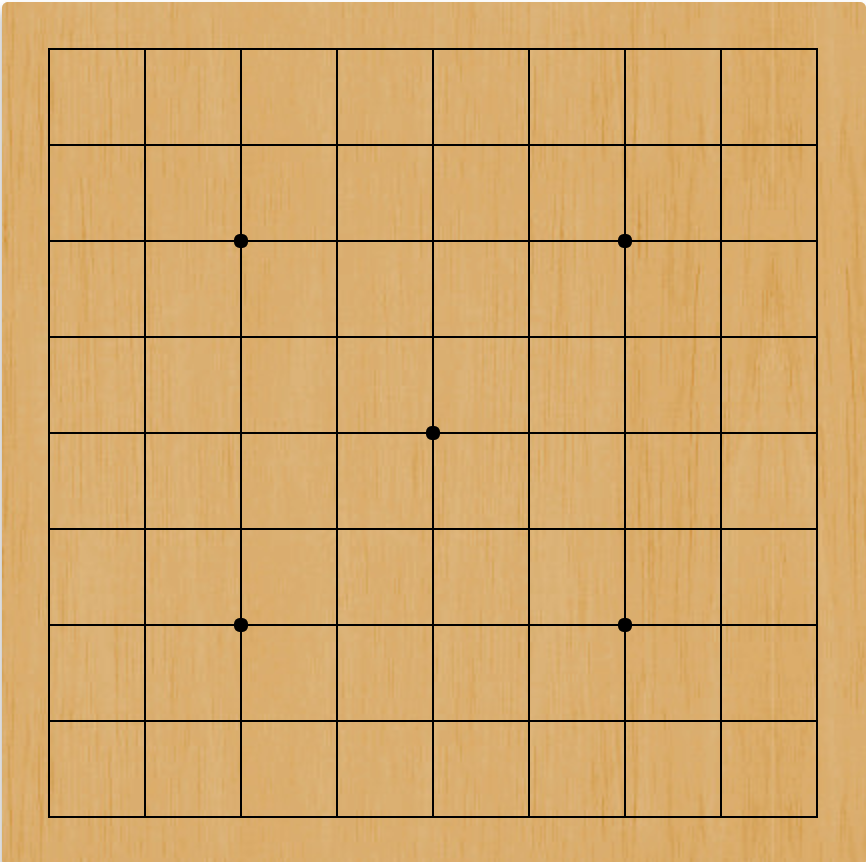
\includegraphics[width=0.4\textwidth]{figs/gorule1.png} }
      \only<2> { 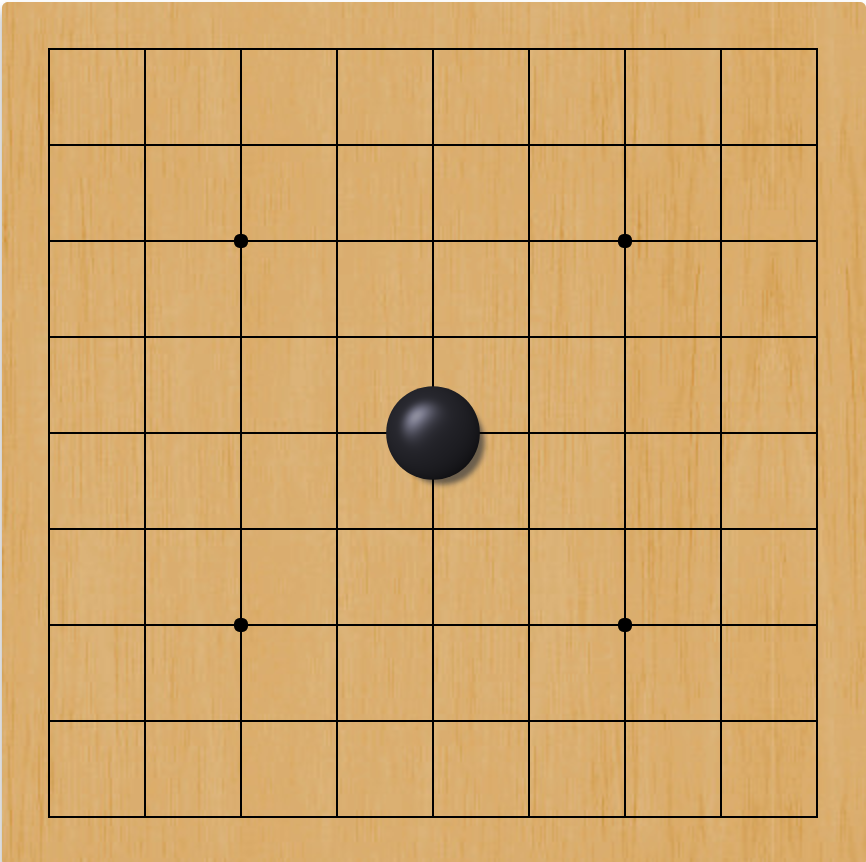
\includegraphics[width=0.4\textwidth]{figs/gorule2.png} }
      \only<3> { 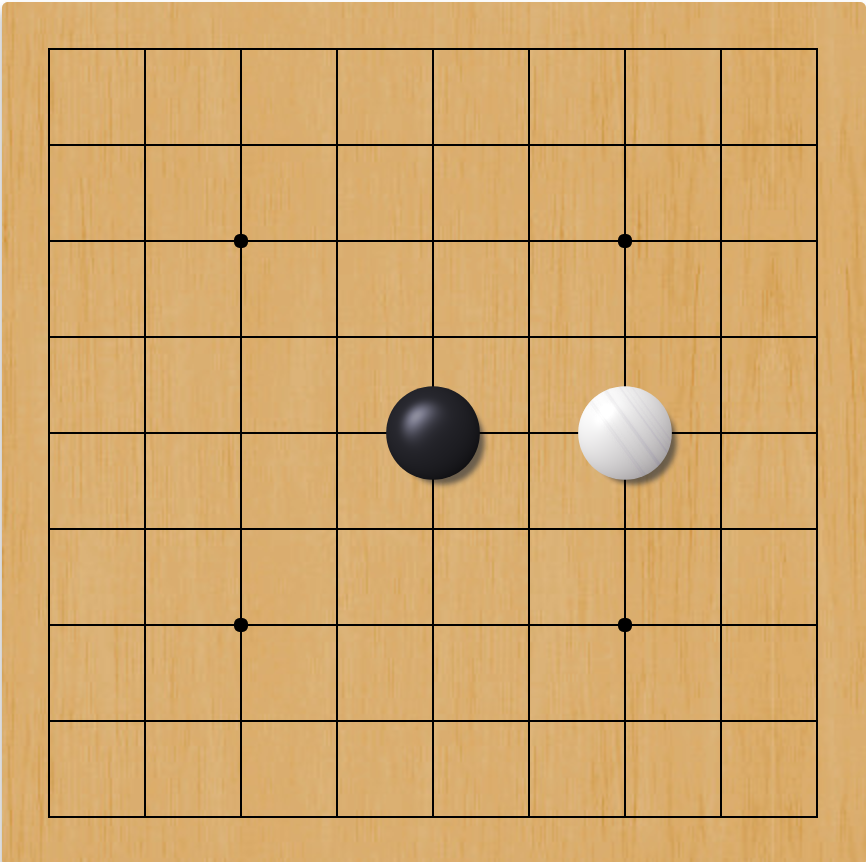
\includegraphics[width=0.4\textwidth]{figs/gorule3.png} }
      \only<4> { 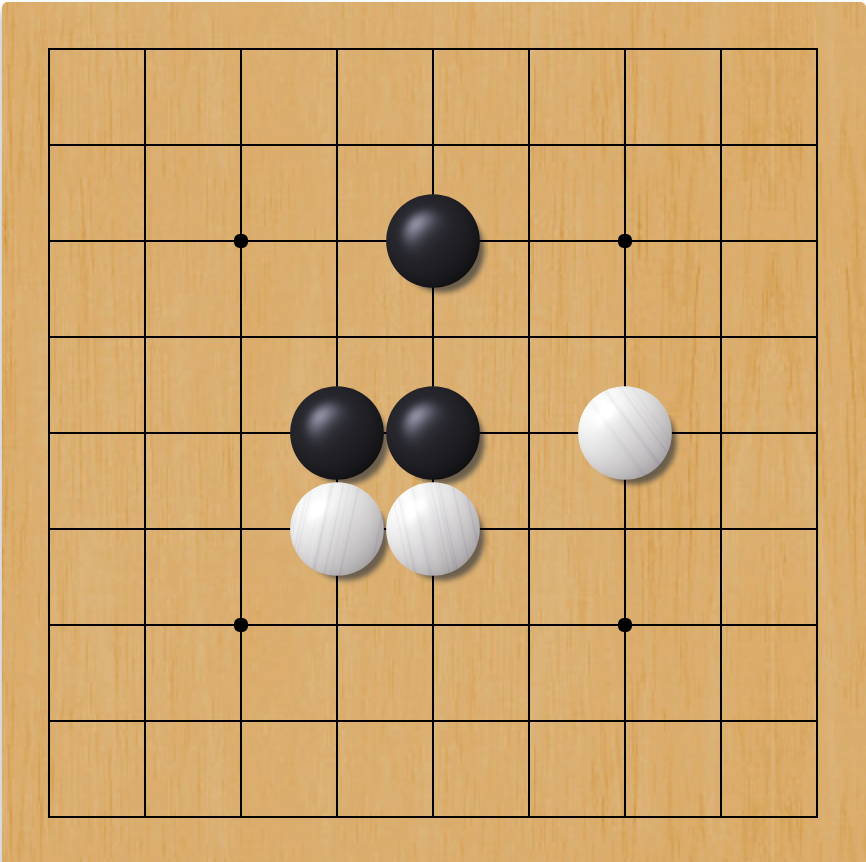
\includegraphics[width=0.4\textwidth]{figs/gorule4.png} }
  \end{center}


}

\frame{
  \frametitle{Règles: chaînes et libertés}

  \begin{itemize}
      \item Pierres reliées horizontalement ou verticalement: \textbf{une chaine}
      \item Emplacements libres autour d'une chaine: \textbf{liberté}
  \end{itemize}

  \begin{center}
      \only<1> { 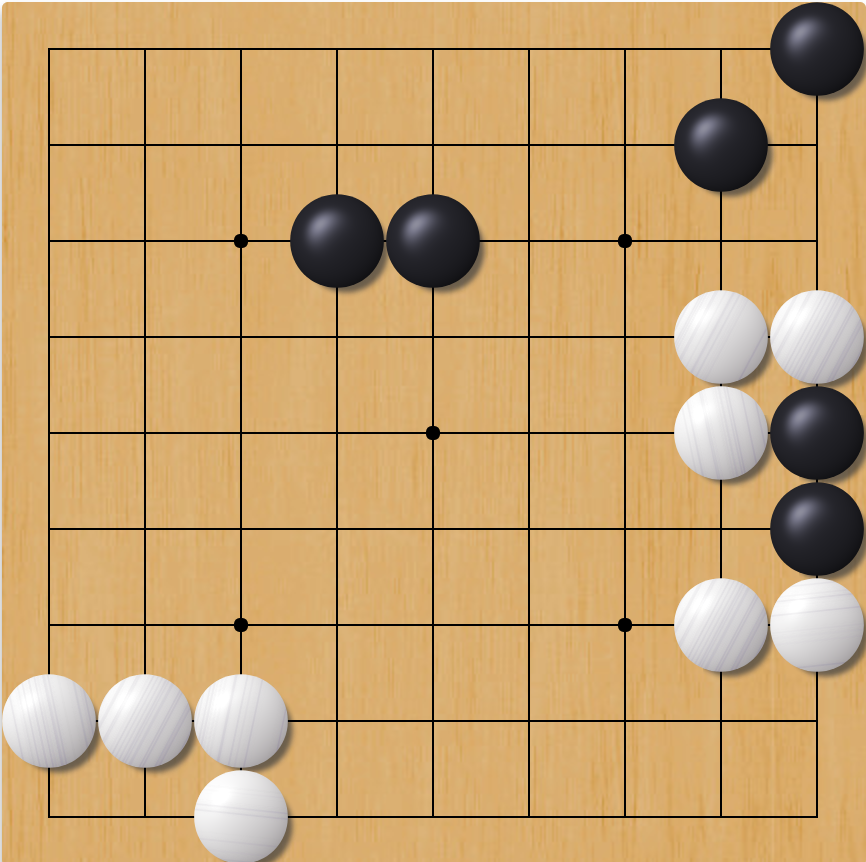
\includegraphics[width=0.4\textwidth]{figs/gorule_string1.png} }
      \only<2> { 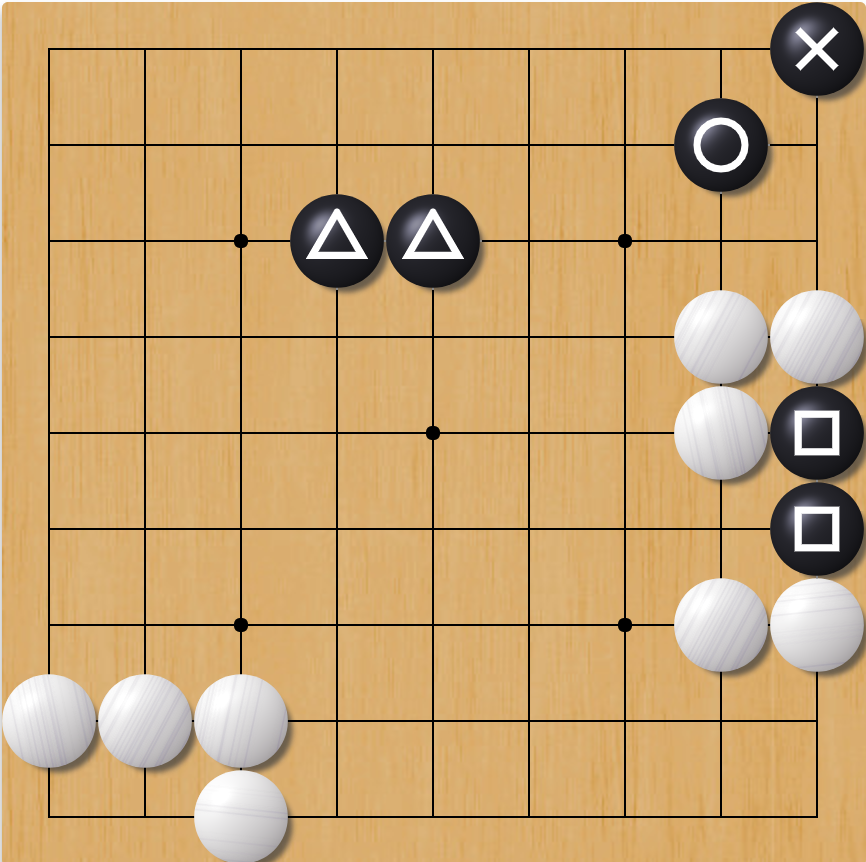
\includegraphics[width=0.4\textwidth]{figs/gorule_string2.png} }
      \only<3> { 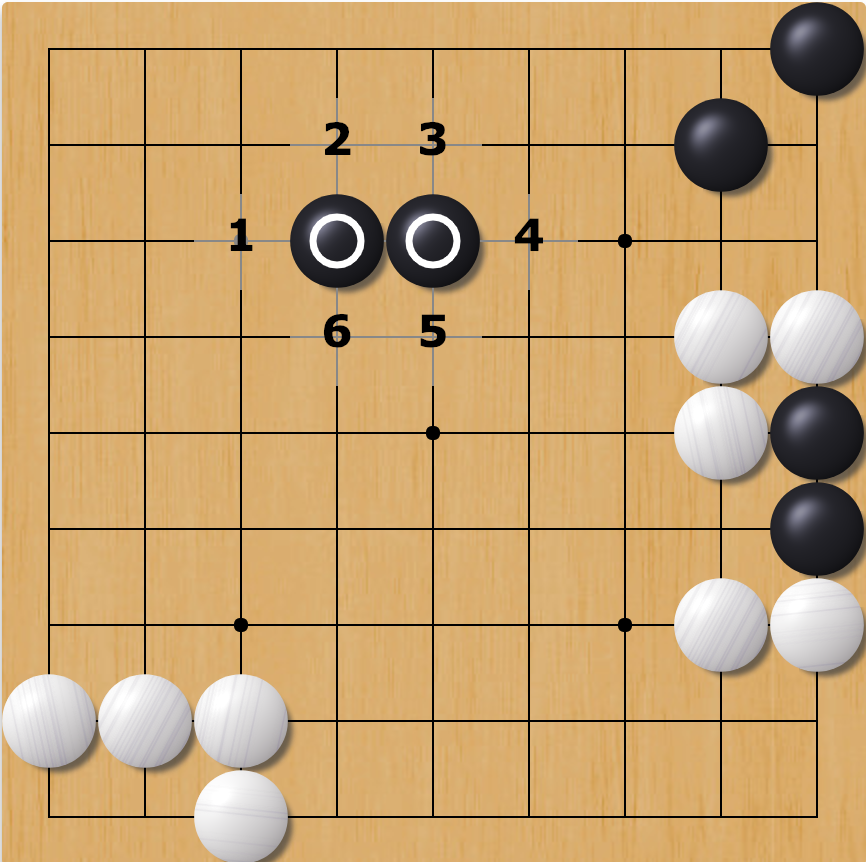
\includegraphics[width=0.4\textwidth]{figs/gorule_string3.png} }
      \only<4> { 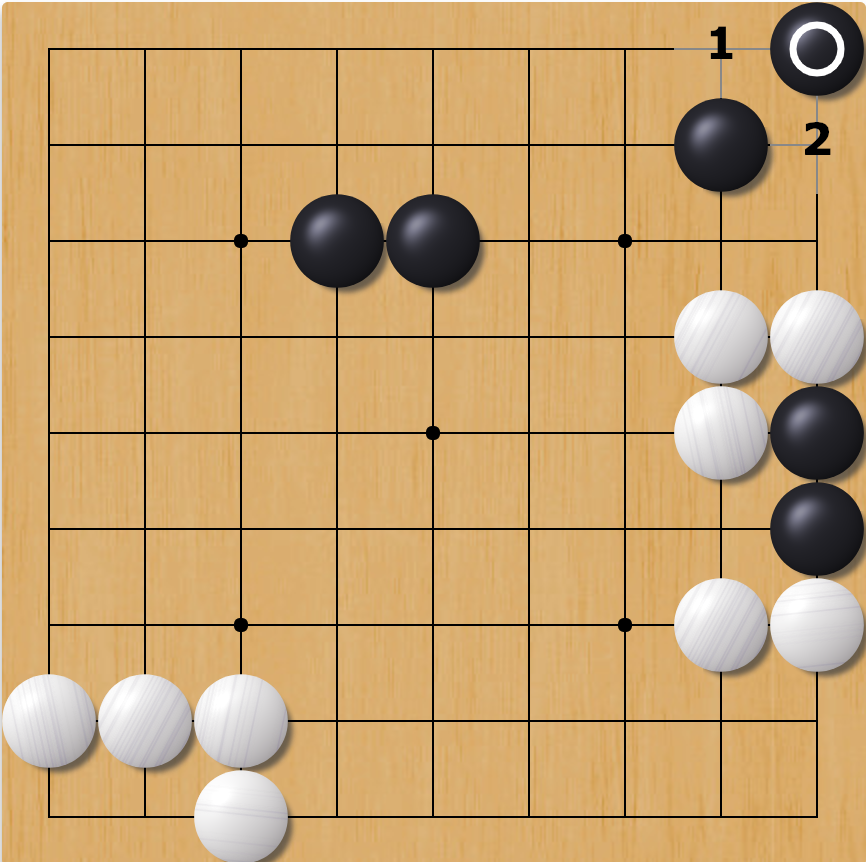
\includegraphics[width=0.4\textwidth]{figs/gorule_string4.png} }
      \only<5> { 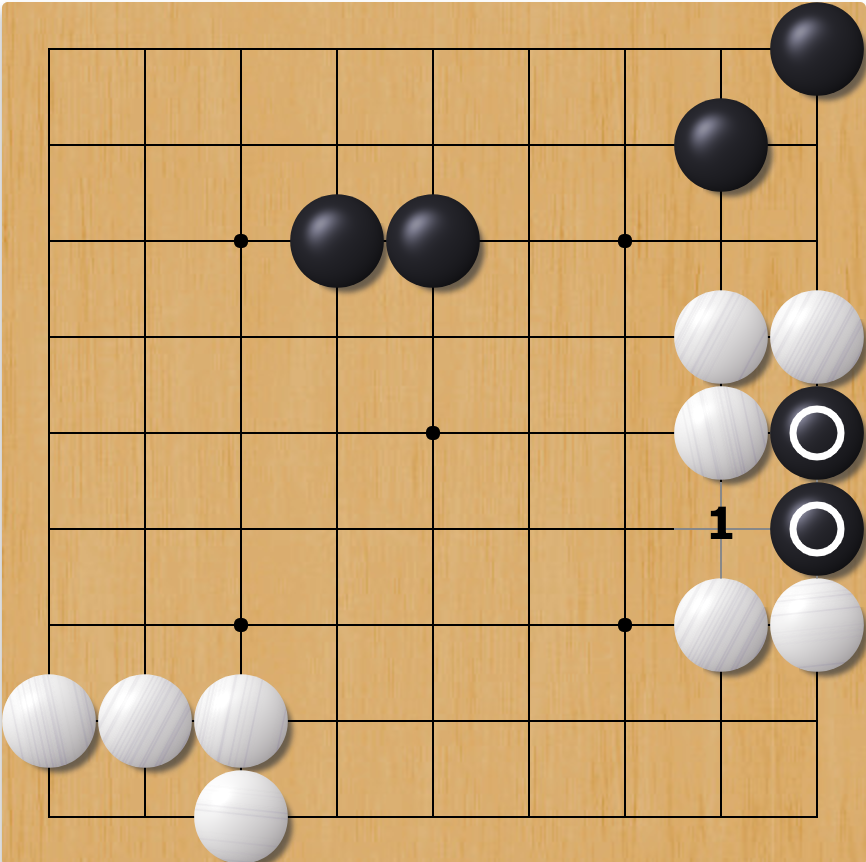
\includegraphics[width=0.4\textwidth]{figs/gorule_string5.png} }
      \only<6> { 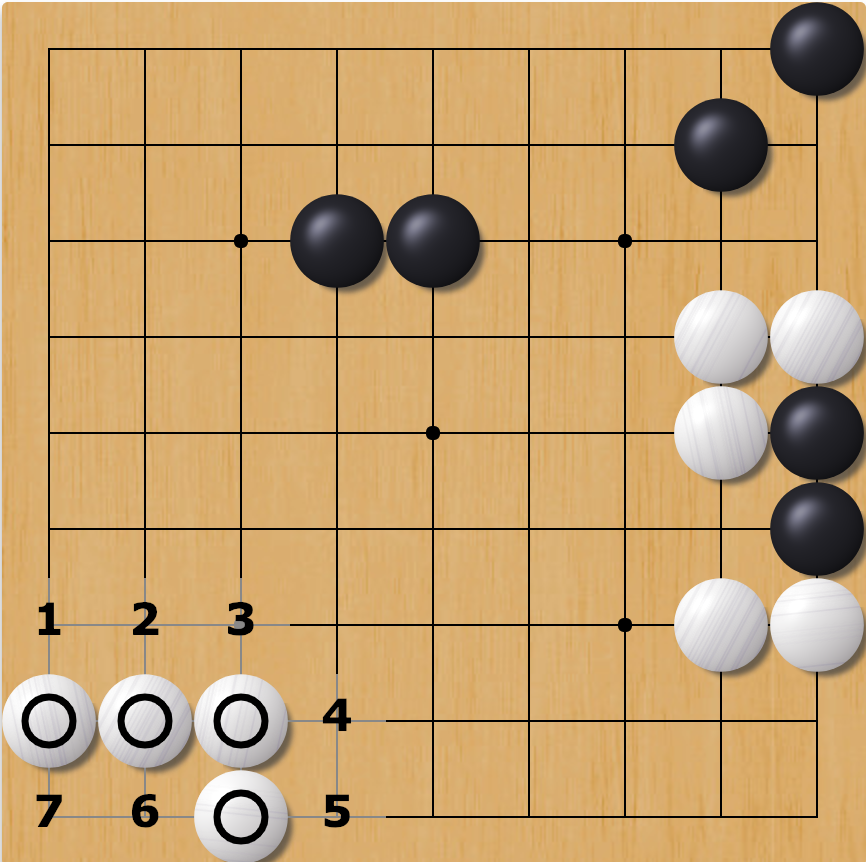
\includegraphics[width=0.4\textwidth]{figs/gorule_string6.png} }
  \end{center}

}

\frame{
  \frametitle{Règles: capture}

  \begin{itemize}
      \item Enlever la dernière liberté d'une chaine: \textbf{capture}
      \itemSo les pierres sont enlevées du plateau
  \end{itemize}

  \begin{center}
      \only<1> { 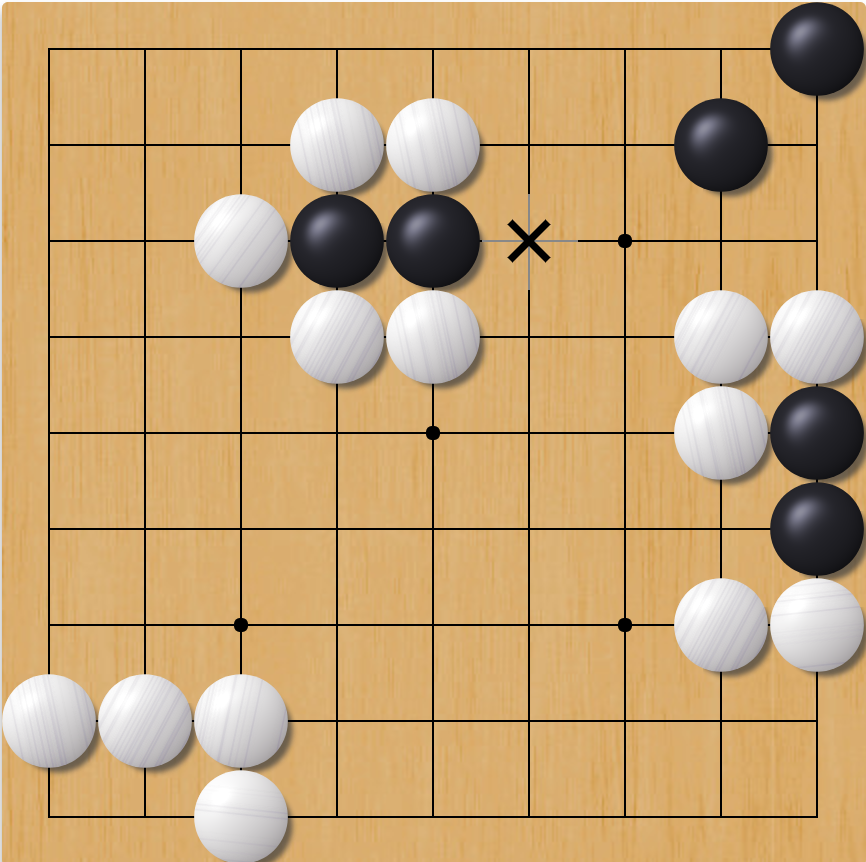
\includegraphics[width=0.4\textwidth]{figs/gorule_capture1.png} }
      \only<2> { 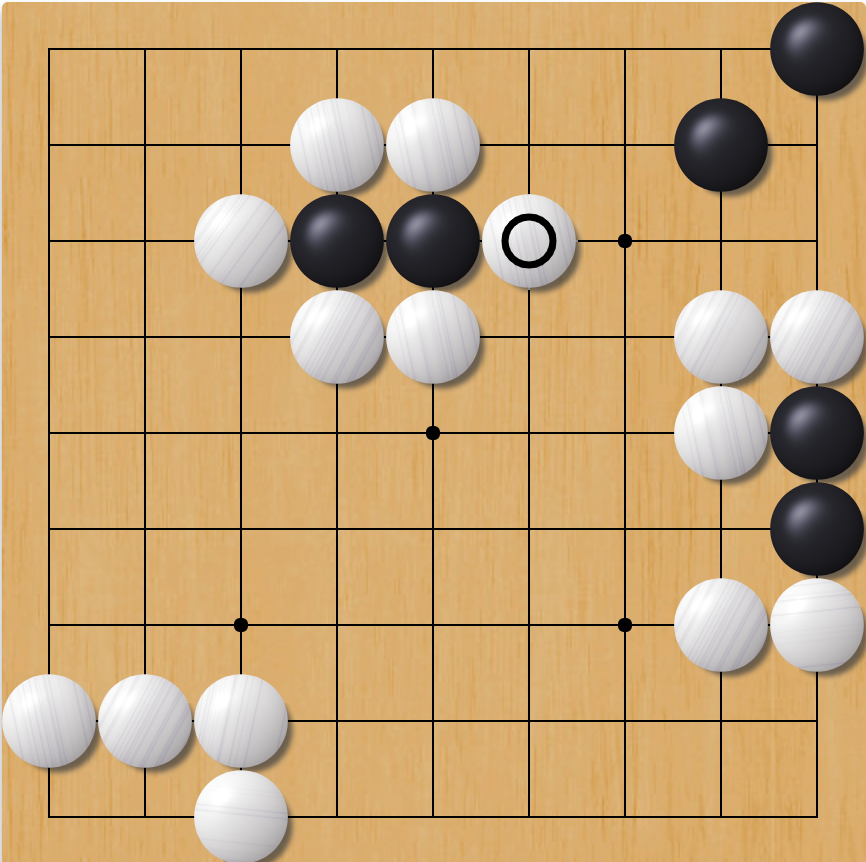
\includegraphics[width=0.4\textwidth]{figs/gorule_capture2.png} }
      \only<3> { 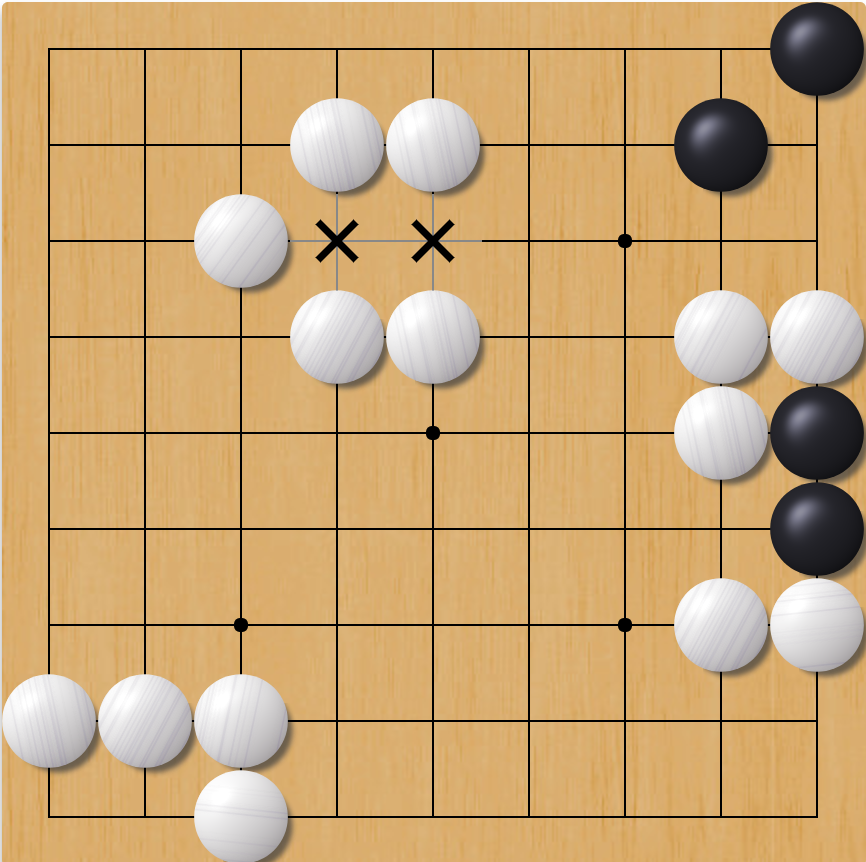
\includegraphics[width=0.4\textwidth]{figs/gorule_capture3.png} }
      \only<4> { 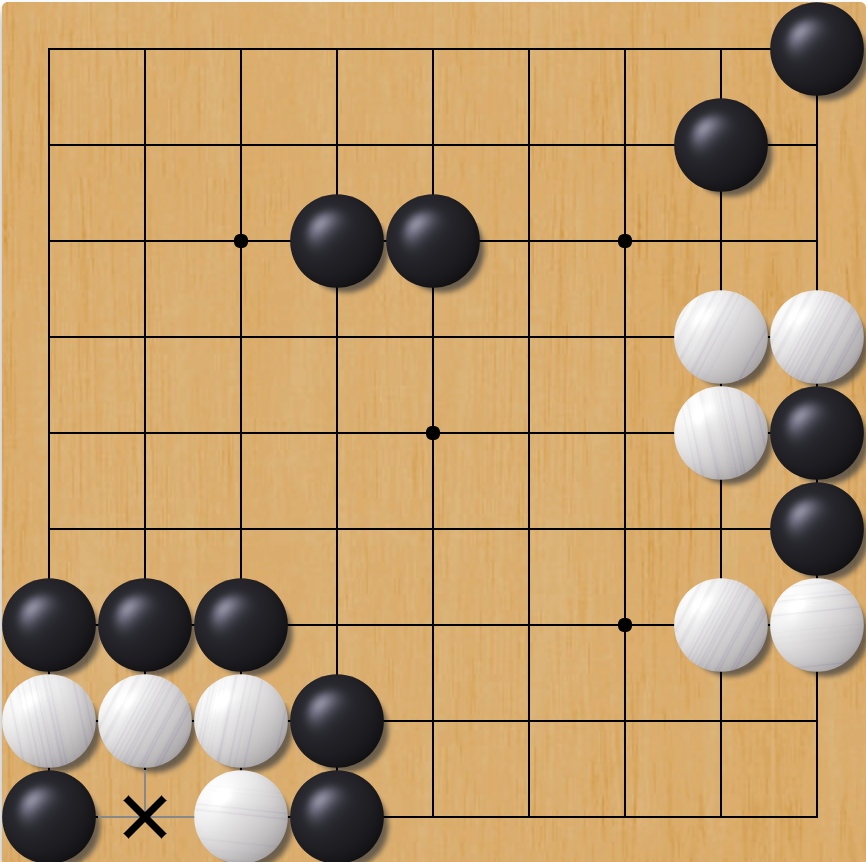
\includegraphics[width=0.4\textwidth]{figs/gorule_capture4.png} }
      \only<5> { 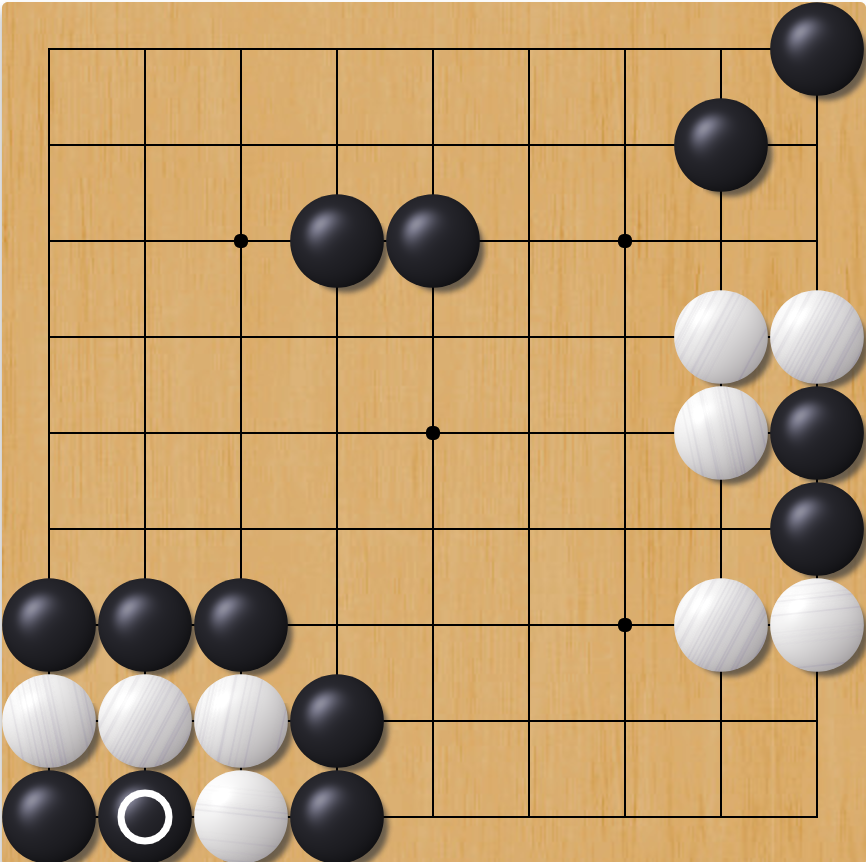
\includegraphics[width=0.4\textwidth]{figs/gorule_capture5.png} }
      \only<6> { 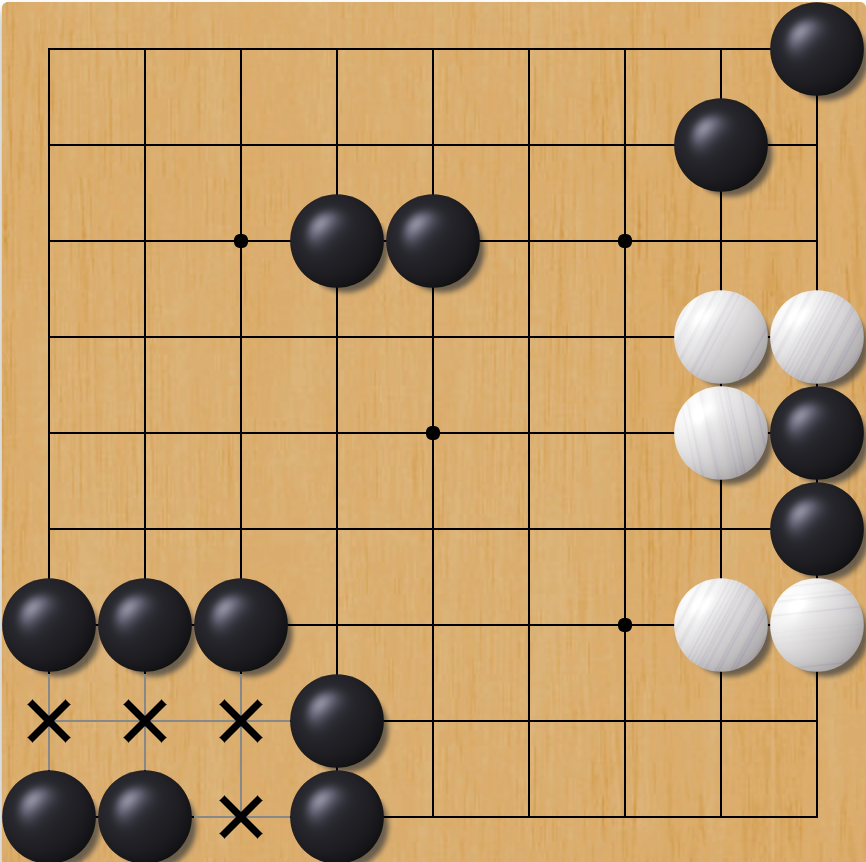
\includegraphics[width=0.4\textwidth]{figs/gorule_capture6.png} }
  \end{center}

}

\frame{
  \frametitle{Règles: fin de partie}

  \begin{itemize}
      \item partie terminée quand les deux joueurs passent
      \item score: pierres + territoire
  \end{itemize}

  \begin{center}
      \only<1> { 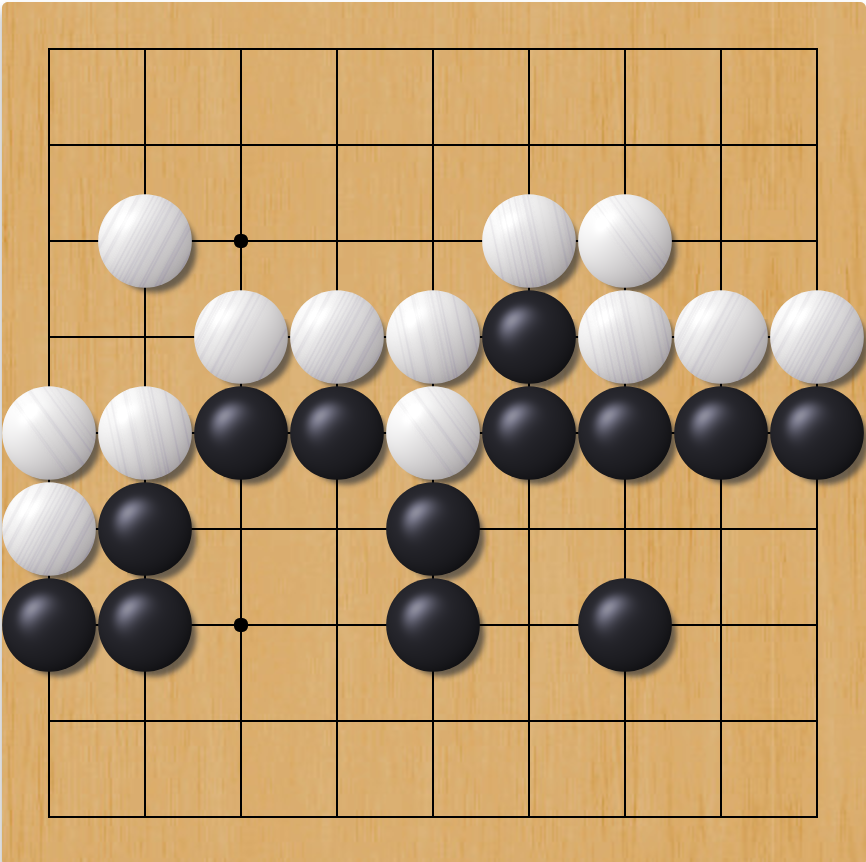
\includegraphics[width=0.4\textwidth]{figs/gorule_score1.png} }
      \only<2> { 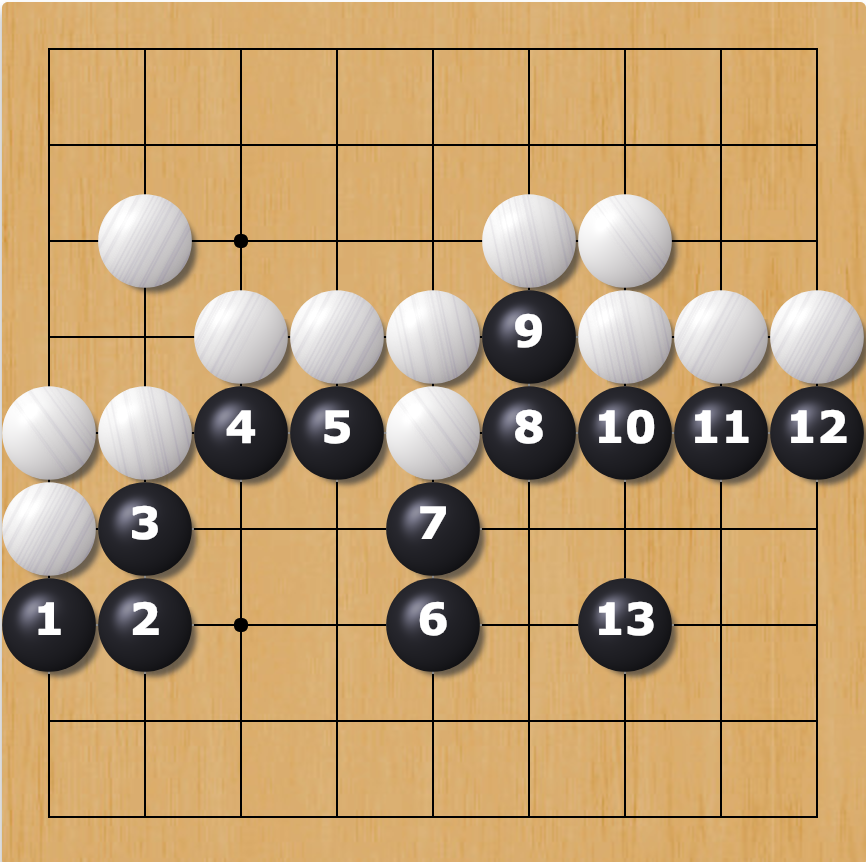
\includegraphics[width=0.4\textwidth]{figs/gorule_score2.png} }
      \only<3> { 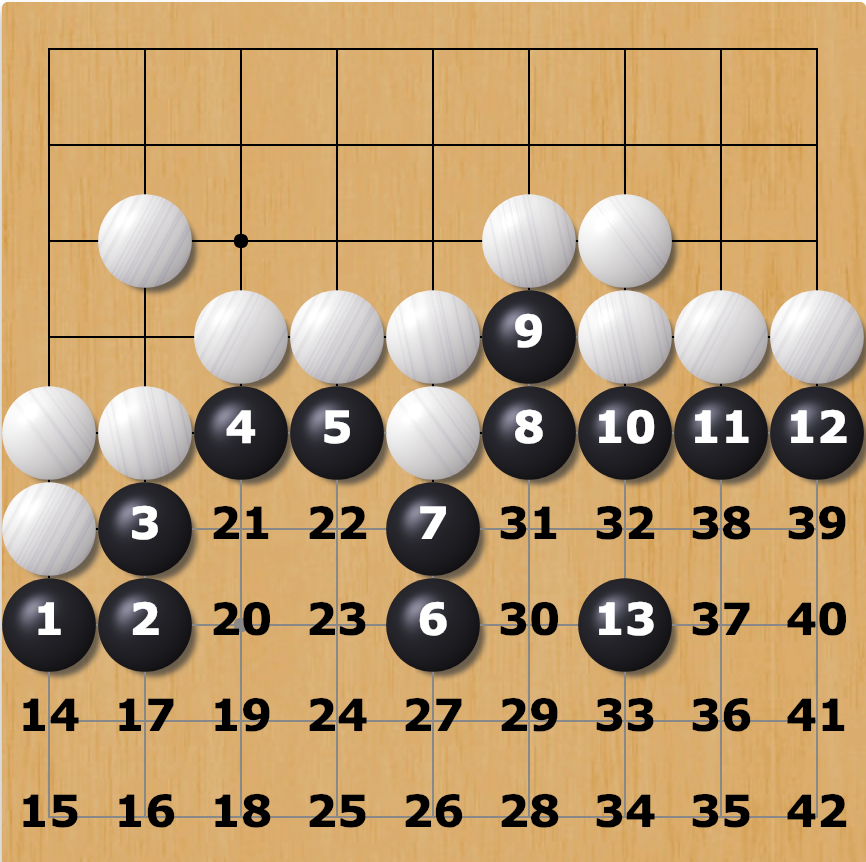
\includegraphics[width=0.4\textwidth]{figs/gorule_score3.png} }
      \only<4> { 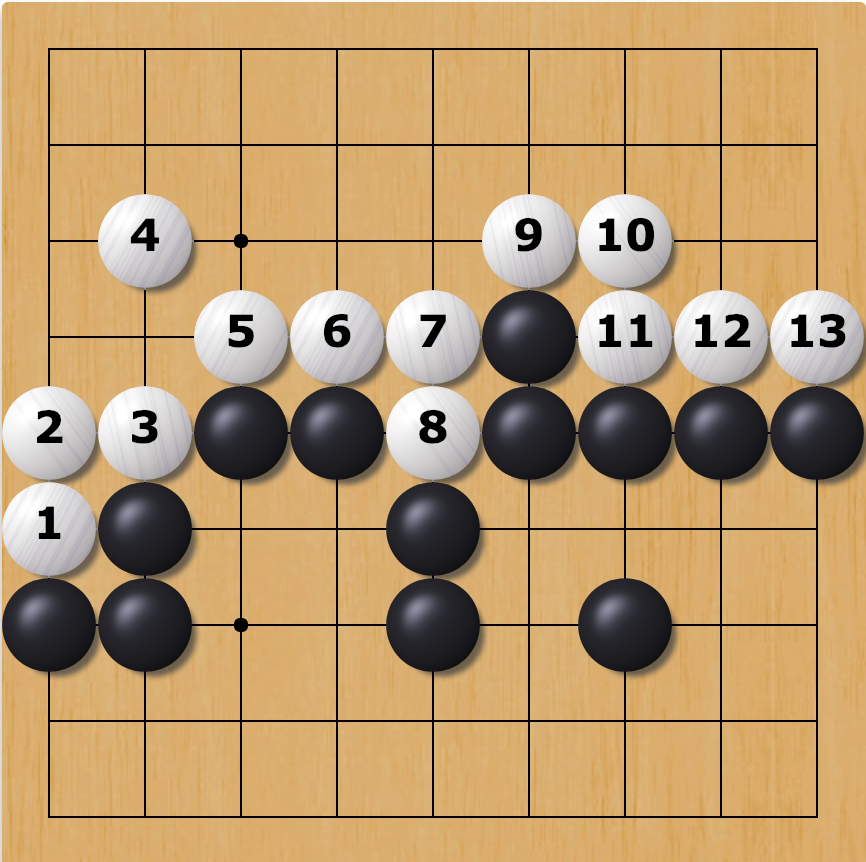
\includegraphics[width=0.4\textwidth]{figs/gorule_score4.png} }
      \only<5> { 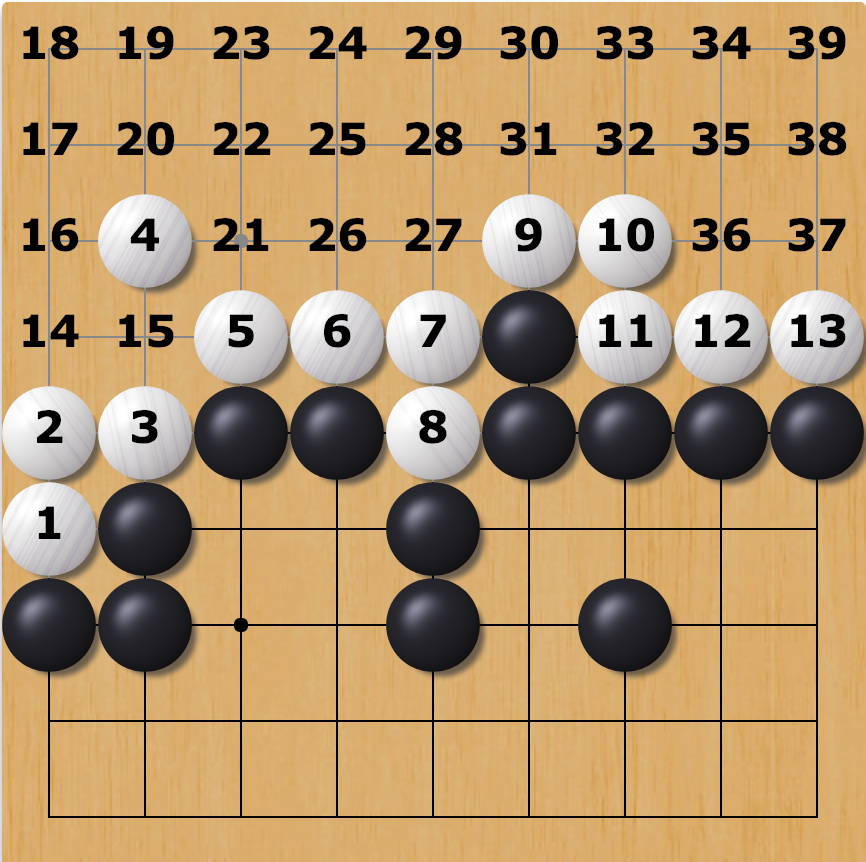
\includegraphics[width=0.4\textwidth]{figs/gorule_score5.png} }
  \end{center}
  TODO score

}

\frame{
  \frametitle{Règles: le ko}


  \begin{center}
      \only<1> { 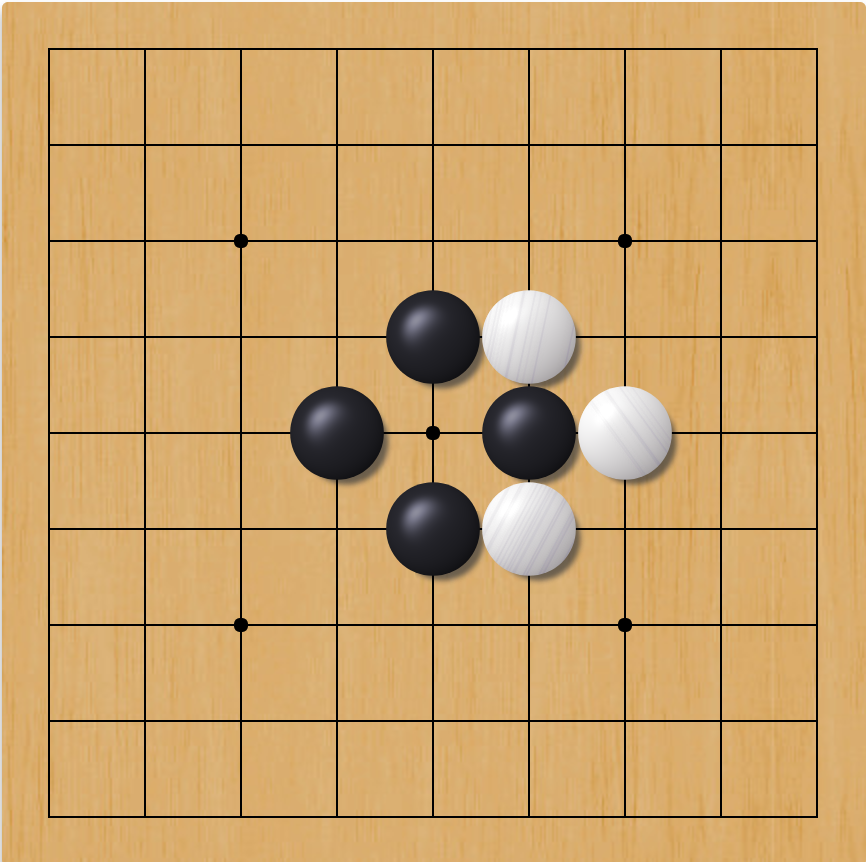
\includegraphics[width=0.4\textwidth]{figs/gorule_ko1.png} }
      \only<2> { 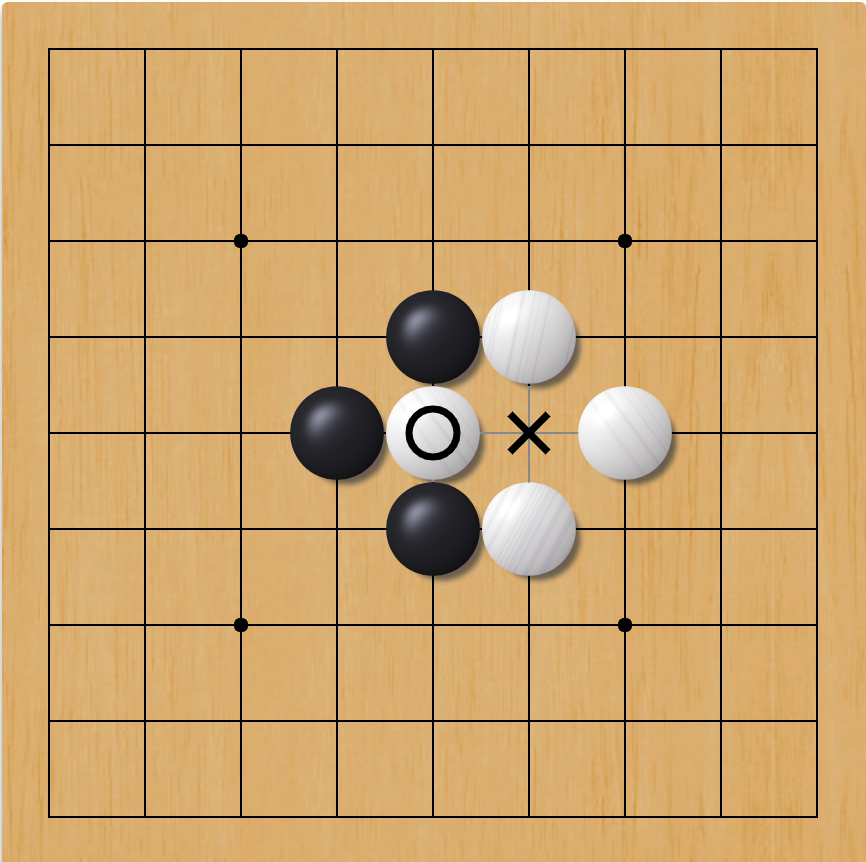
\includegraphics[width=0.4\textwidth]{figs/gorule_ko2.png} }
      \only<3> { 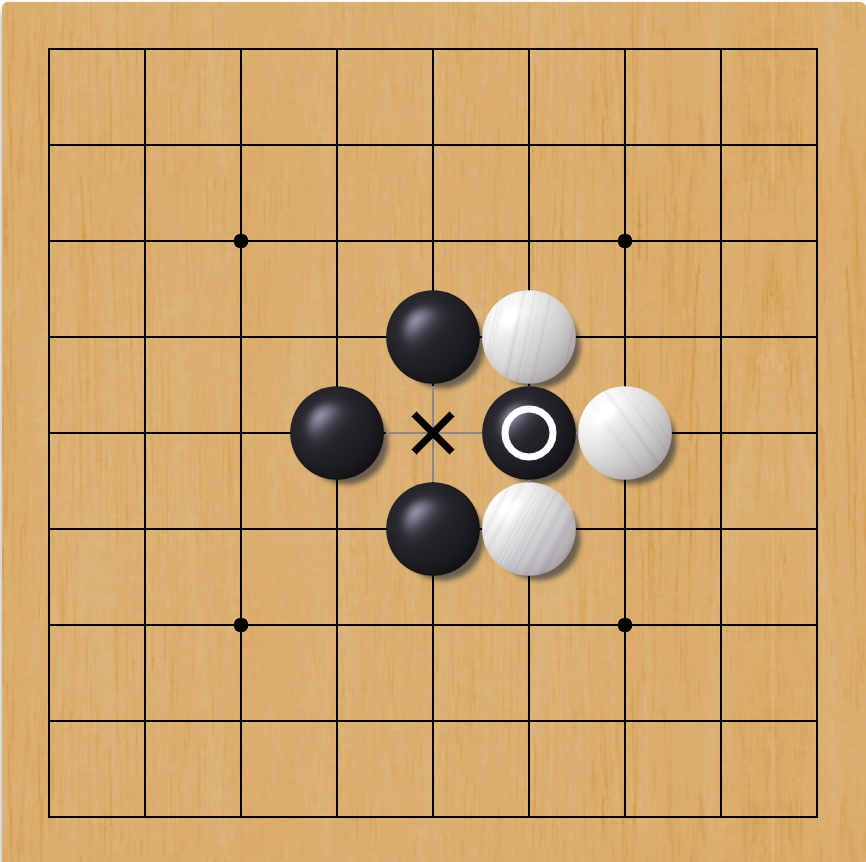
\includegraphics[width=0.4\textwidth]{figs/gorule_ko3.png} }
  \end{center}
  \begin{itemize}
      \item problème: captures répétées successives
      \item règle (humain): pas le droit de remettre le plateau dans l'état juste avant
      \item règle (ordinateur): pas le droit de remettre le plateau dans n'importe quel état précédant
  \end{itemize}



}

\frame{
  \frametitle{Echelle de niveau}


  TODO tikz
}

\section{Avant l'Exploration d'Arbre par Bandit}

\frame{
  \frametitle{Principe}

  \begin{itemize}
      \item Exploration d'arbre \red{alphabeta}
      \item Evaluation des noeuds basée sur des \red{connaissances expertes}
  \end{itemize}

  \begin{center}
    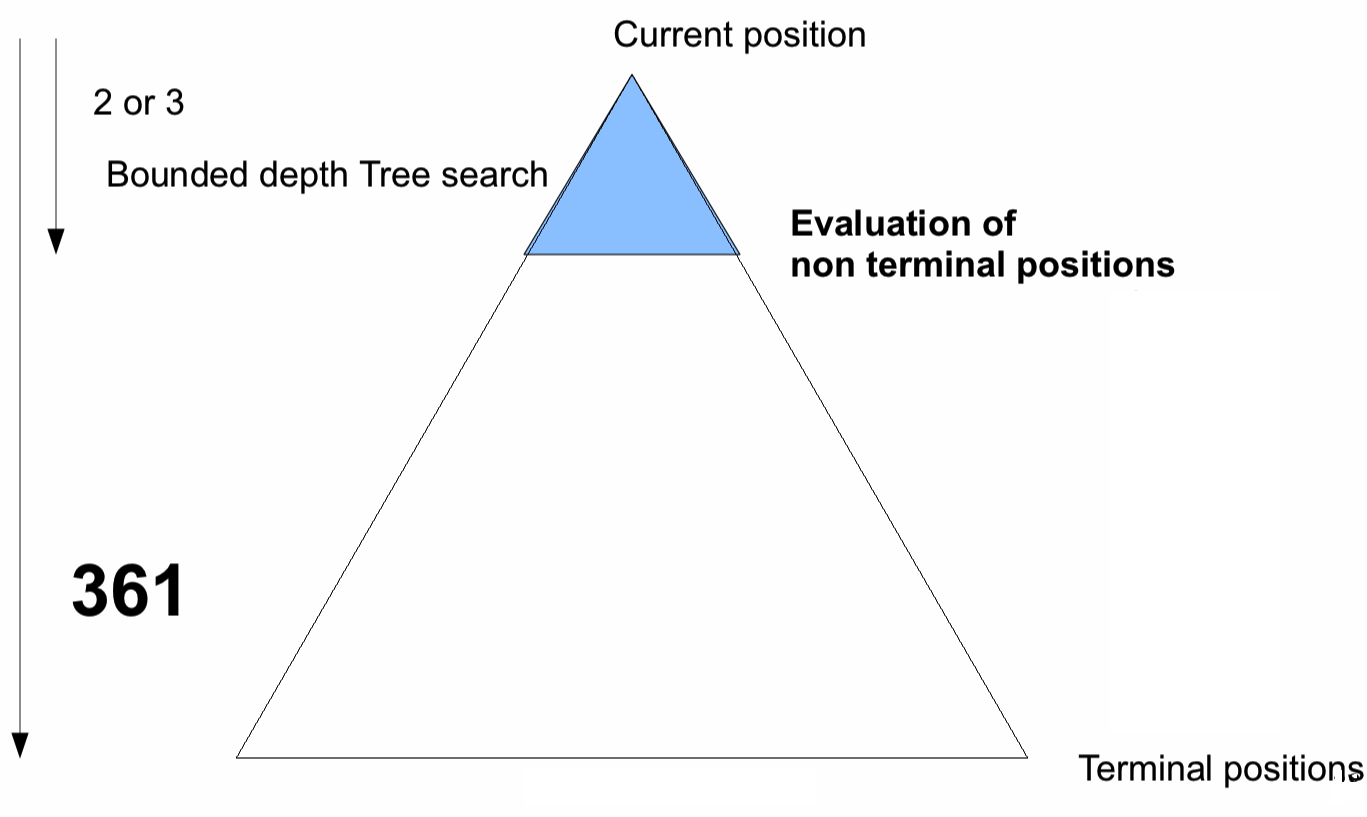
\includegraphics[width=0.8\textwidth]{figs/alphabetago.png}
  \end{center}

}

\frame{
  \frametitle{Evaluation}

  \begin{itemize}
      \item \red{Découpage} du plateau en sous parties
      \item \red{Evaluation} de chaque sous partie par \textbf{recherche locale} (souvent alphabeta)
      \itemSo groupe mort, vivant, territoire, ...
      \item \red{Recomposition} d'un score global
  \end{itemize}


}

\frame{
  \frametitle{Position à évaluer}

  \begin{center}
    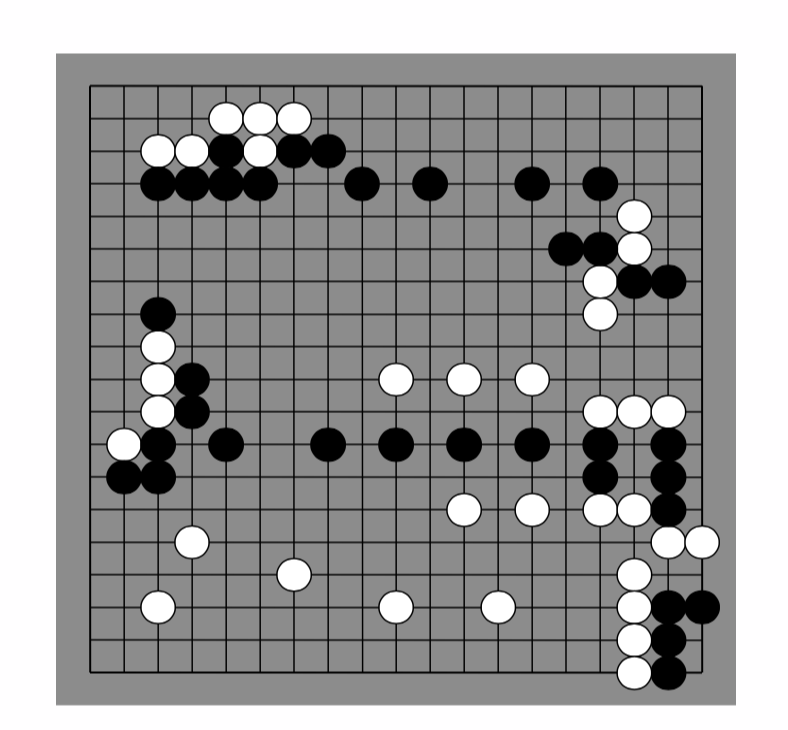
\includegraphics[width=0.7\textwidth]{figs/alphabeta_poseval.png}
  \end{center}

}

\frame{
  \frametitle{Découpage du plateau}

  \begin{center}
    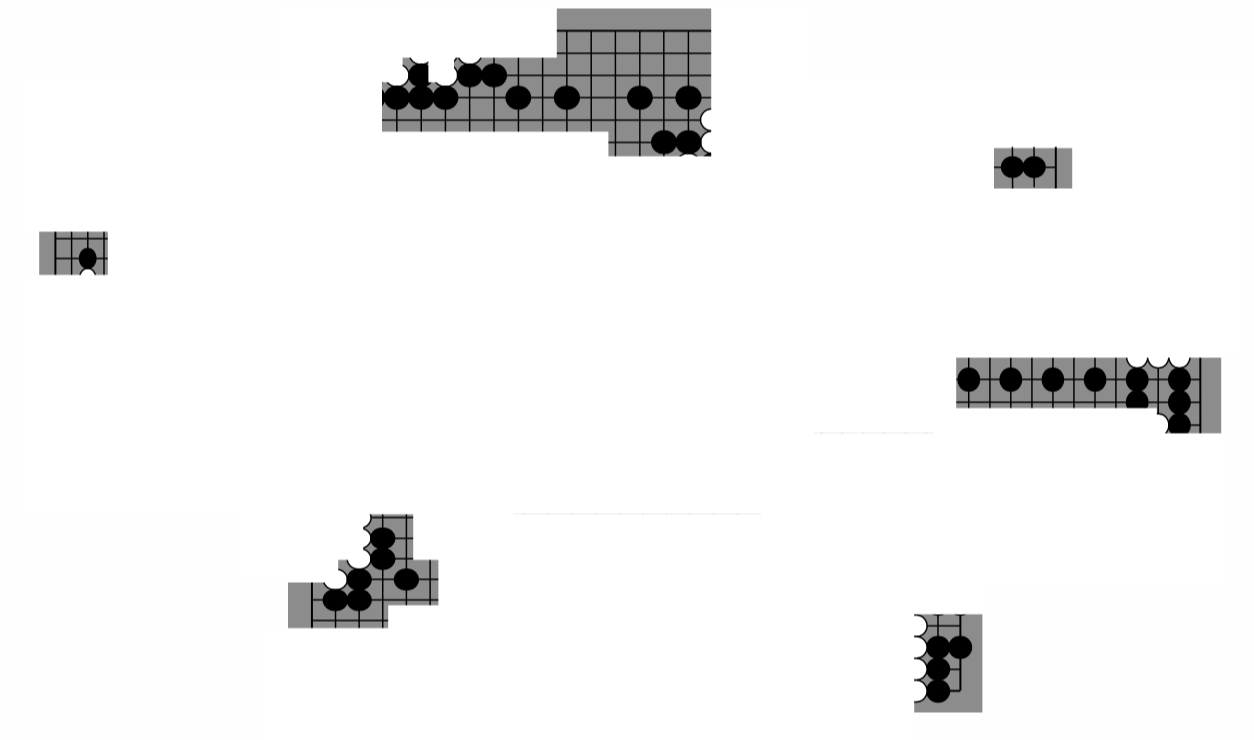
\includegraphics[width=0.8\textwidth]{figs/alphabeta_decoupage.png}
  \end{center}

}

\frame{
  \frametitle{Evaluation locale}

  \begin{center}
    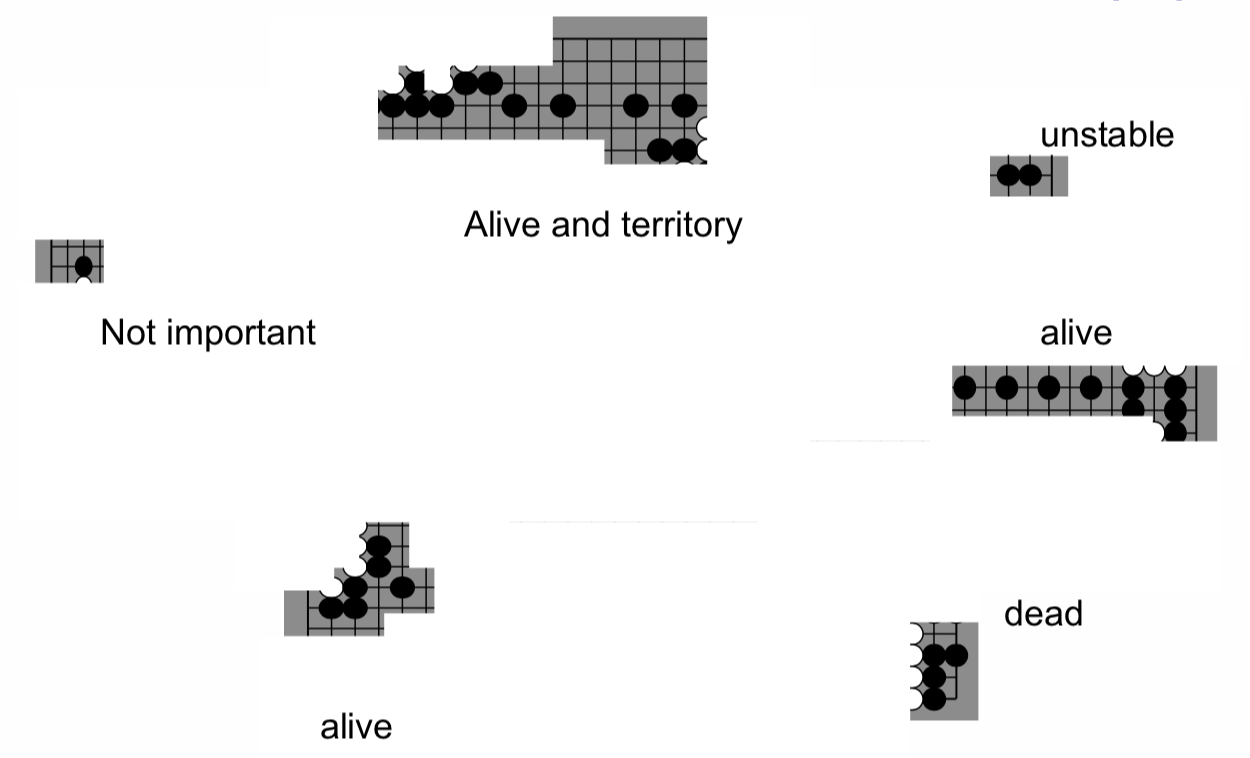
\includegraphics[width=0.8\textwidth]{figs/alphabeta_but.png}
  \end{center}

}

\frame{
  \frametitle{Evaluation globale}

  \begin{center}
    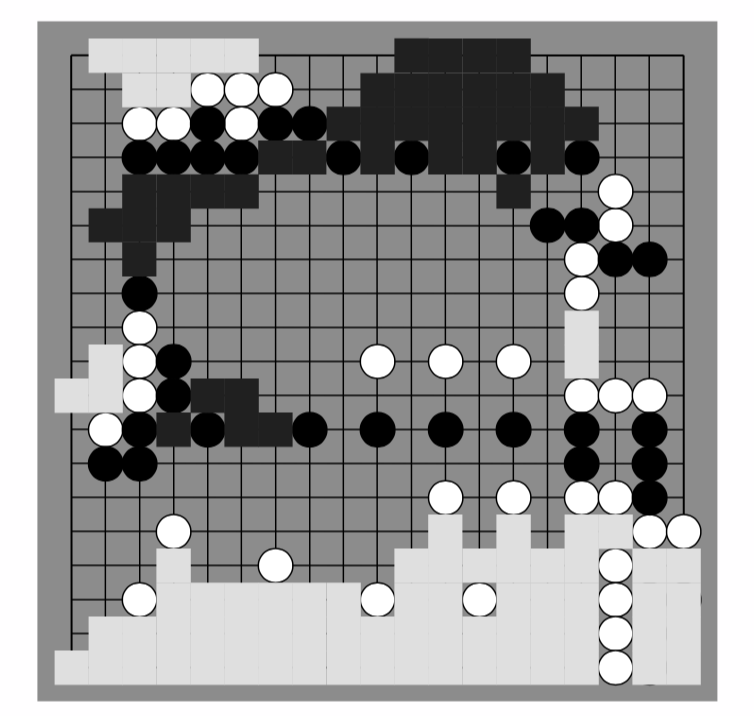
\includegraphics[width=0.7\textwidth]{figs/alphabeta_globaleval.png}
  \end{center}

}


\frame{
  \frametitle{Avantages}

  \begin{itemize}
      \item Algorithme \red{très rapide}
      \item Evaluation locale peut être très performante
  \end{itemize}

}

\frame{
  \frametitle{Inconvénients}

  \begin{itemize}
      \item Découpage et recomposition difficile et ayant un fort impact
      \item Pas d'\textbf{intéraction} entre les positions locales
      \item Demande beaucoup de \textbf{connaissances expertes}
  \end{itemize}

}

\frame{
  \frametitle{Échelle de niveau}

}

\section{Exploration d'Arbre par Bandit}


\subsection{Construction de l'Arbre}

\frame{
  \frametitle{Idée}

  \begin{itemize}
      \item Arbre \red{déséquilibré}
      \itemSo TODO
      \item Construction itérative 
  \end{itemize}

}

\frame{
  \frametitle{Principe}

  \begin{itemize}
      \item Répétition de ces 3 étapes:
          TODO
  \end{itemize}

}

\frame{
  \frametitle{Exemple}

  TODO tikz
}

\frame{
  \frametitle{Questions}

  TODO
  \begin{itemize}
      \item Comment faire l'évaluation?
      \item Comment faire la descente?
  \end{itemize}

}


\subsection{Problème de Bandit}

\begin{frame}
    \frametitle{Introduction du problème}
    \begin{center}
        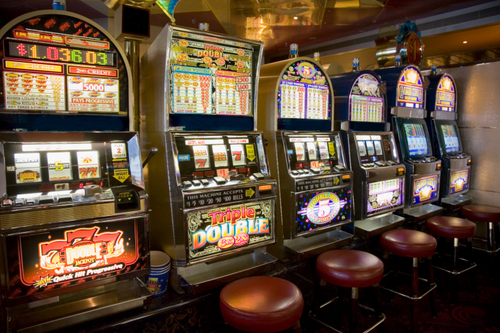
\includegraphics[scale=0.8]{figs/bandit_casino.jpg}
    \end{center}
    Dans un casino, il y a plusieurs machines à sous différentes en terme de récompense.
    \begin{itemize}
        \item Comment répartir mes pièces entre les machines?
    \end{itemize}
\end{frame}

\begin{frame}
    \frametitle{Autres problèmes similaires}
    \begin{center}
        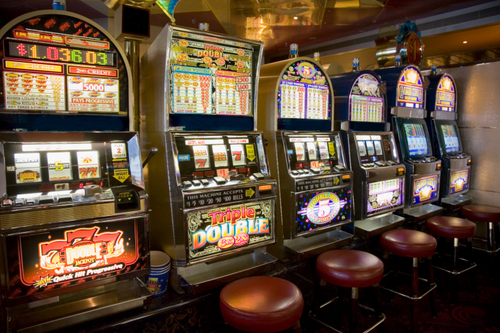
\includegraphics[scale=0.8]{figs/bandit_casino.jpg}
    \end{center}
    \begin{itemize}
        \item Essais cliniques: trouver le traitement qui fonctionne le mieux.
        \item Sélection d'un serveur dans un réseau: trouver le serveur avec le temps de réponse le plus faible.
        \item Publicité ciblée: trouver le type de pub qui intéressera le plus un utilisateur.
        \item ...
    \end{itemize}
    Ce sont des problèmes où on a plusieurs fois le même choix à effectuer. Le choix conduit à une récompense aléatoire.
\end{frame}


\begin{frame}
    \frametitle{Définition formelle}
    \begin{center}
        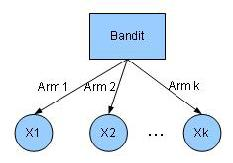
\includegraphics[scale=0.5]{figs/bandit.jpg}
    \end{center}
    \begin{itemize}
        \item un ensemble de bras $A=\{1,...,K\}$.
        \item chaque bras est associé à une distribution de probabilité $X_k$ d'espérance $\mu_k$.
        \item l'algorithme choisit un bras $a$ à chaque pas de temps.
        \item le bandit retourne une récompense $r$ : une réalisation de $X_a$.
        \item les tirages successifs sur un même bras sont indépendant et identiquement distribués.
    \end{itemize}
\end{frame}



\begin{frame}
    \frametitle{Notations supplémentaires}
    \begin{itemize}
        \item $T_i(n)$: le nombre de fois que le bras $i$ a été sélectionné au pas de temps $n$.
        \item $\mu^* = \max_{1 \le i \le K}\mu_i$
        \item $\Delta_i = \mu^* - \mu_i$ 
        \item $\Delta = \min_{i:\Delta_i > 0}\Delta_i$
    \end{itemize}


\end{frame}


\begin{frame}
    \frametitle{Objectif}

    Le but est d'optimiser le regret $R_n$ défini comme suit:

    $$R_n=\mu^*n - \mathbb{E} \sum_{j=1}^{K}  T_j(n) \mu_j$$
    $$R_n=\sum_{j=1}^{K} \Delta_j \mathbb{E} [T_j(n)]$$

\end{frame}



\begin{frame}
    \frametitle{Borne inférieure}


    Pour toute stratégie d'allocation et pour tout bras non optimal:
    $$\mathbb{E} [T_j(n)] \ge \frac{\log n}{D(p_j || p^*)}$$

    $$\mbox{où }D(p_j || p^*) = \int p_j \log \frac{p_j}{p^*}$$
    On en déduit que le meilleur regret atteignable est en ${\color{red} \log(n)}$.

    \hfill [Lai and Robbins, 1985]

\end{frame}



\begin{frame}
    \frametitle{UCB}
    Principe de l'algorithme:
    \begin{itemize}
        \item A partir des informations disponibles au temps $t$, on calcule la borne de confiance supérieur (UCB) correspondant à chaque bras.
        \item On choisit le bras qui a la valeur UCB la plus grande.
    \end{itemize}
    \hfill [Auer and all, 2002]
\end{frame}

\begin{frame}
    \frametitle{UCB}
    Calcul de la valeur UCB pour le bras $i$ au pas de temps $t$:
    $$ {\color{red} \hat{\mu}_{i,t-1}} + {\color{green} \sqrt{\frac{3\log(t)}{2T_i(t-1)}}} $$
    où $\hat{\mu}_{i,t-1} $ correspond à la moyenne empirique du bras $i$.
    
\end{frame}

\begin{frame}
    \frametitle{UCB}
    Borne sur le regret:
    $$ R_n \le 6*\sum_{i \ne i^*}\frac{\color{red}\log(n)}{\Delta_i} + K(\frac{\pi^2}{3}+1) $$
    
\end{frame}



\begin{frame}
    \frametitle{Rappel MCTS}

    TODO rappel l'algo
    TODO rappel question: comment faire la descente?


\end{frame}


\begin{frame}
    \frametitle{Descente dans l'arbre}
    La descente dans l'arbre se fait en considérant que chaque choix d'une branche est un problème de bandit.

    \begin{center}
        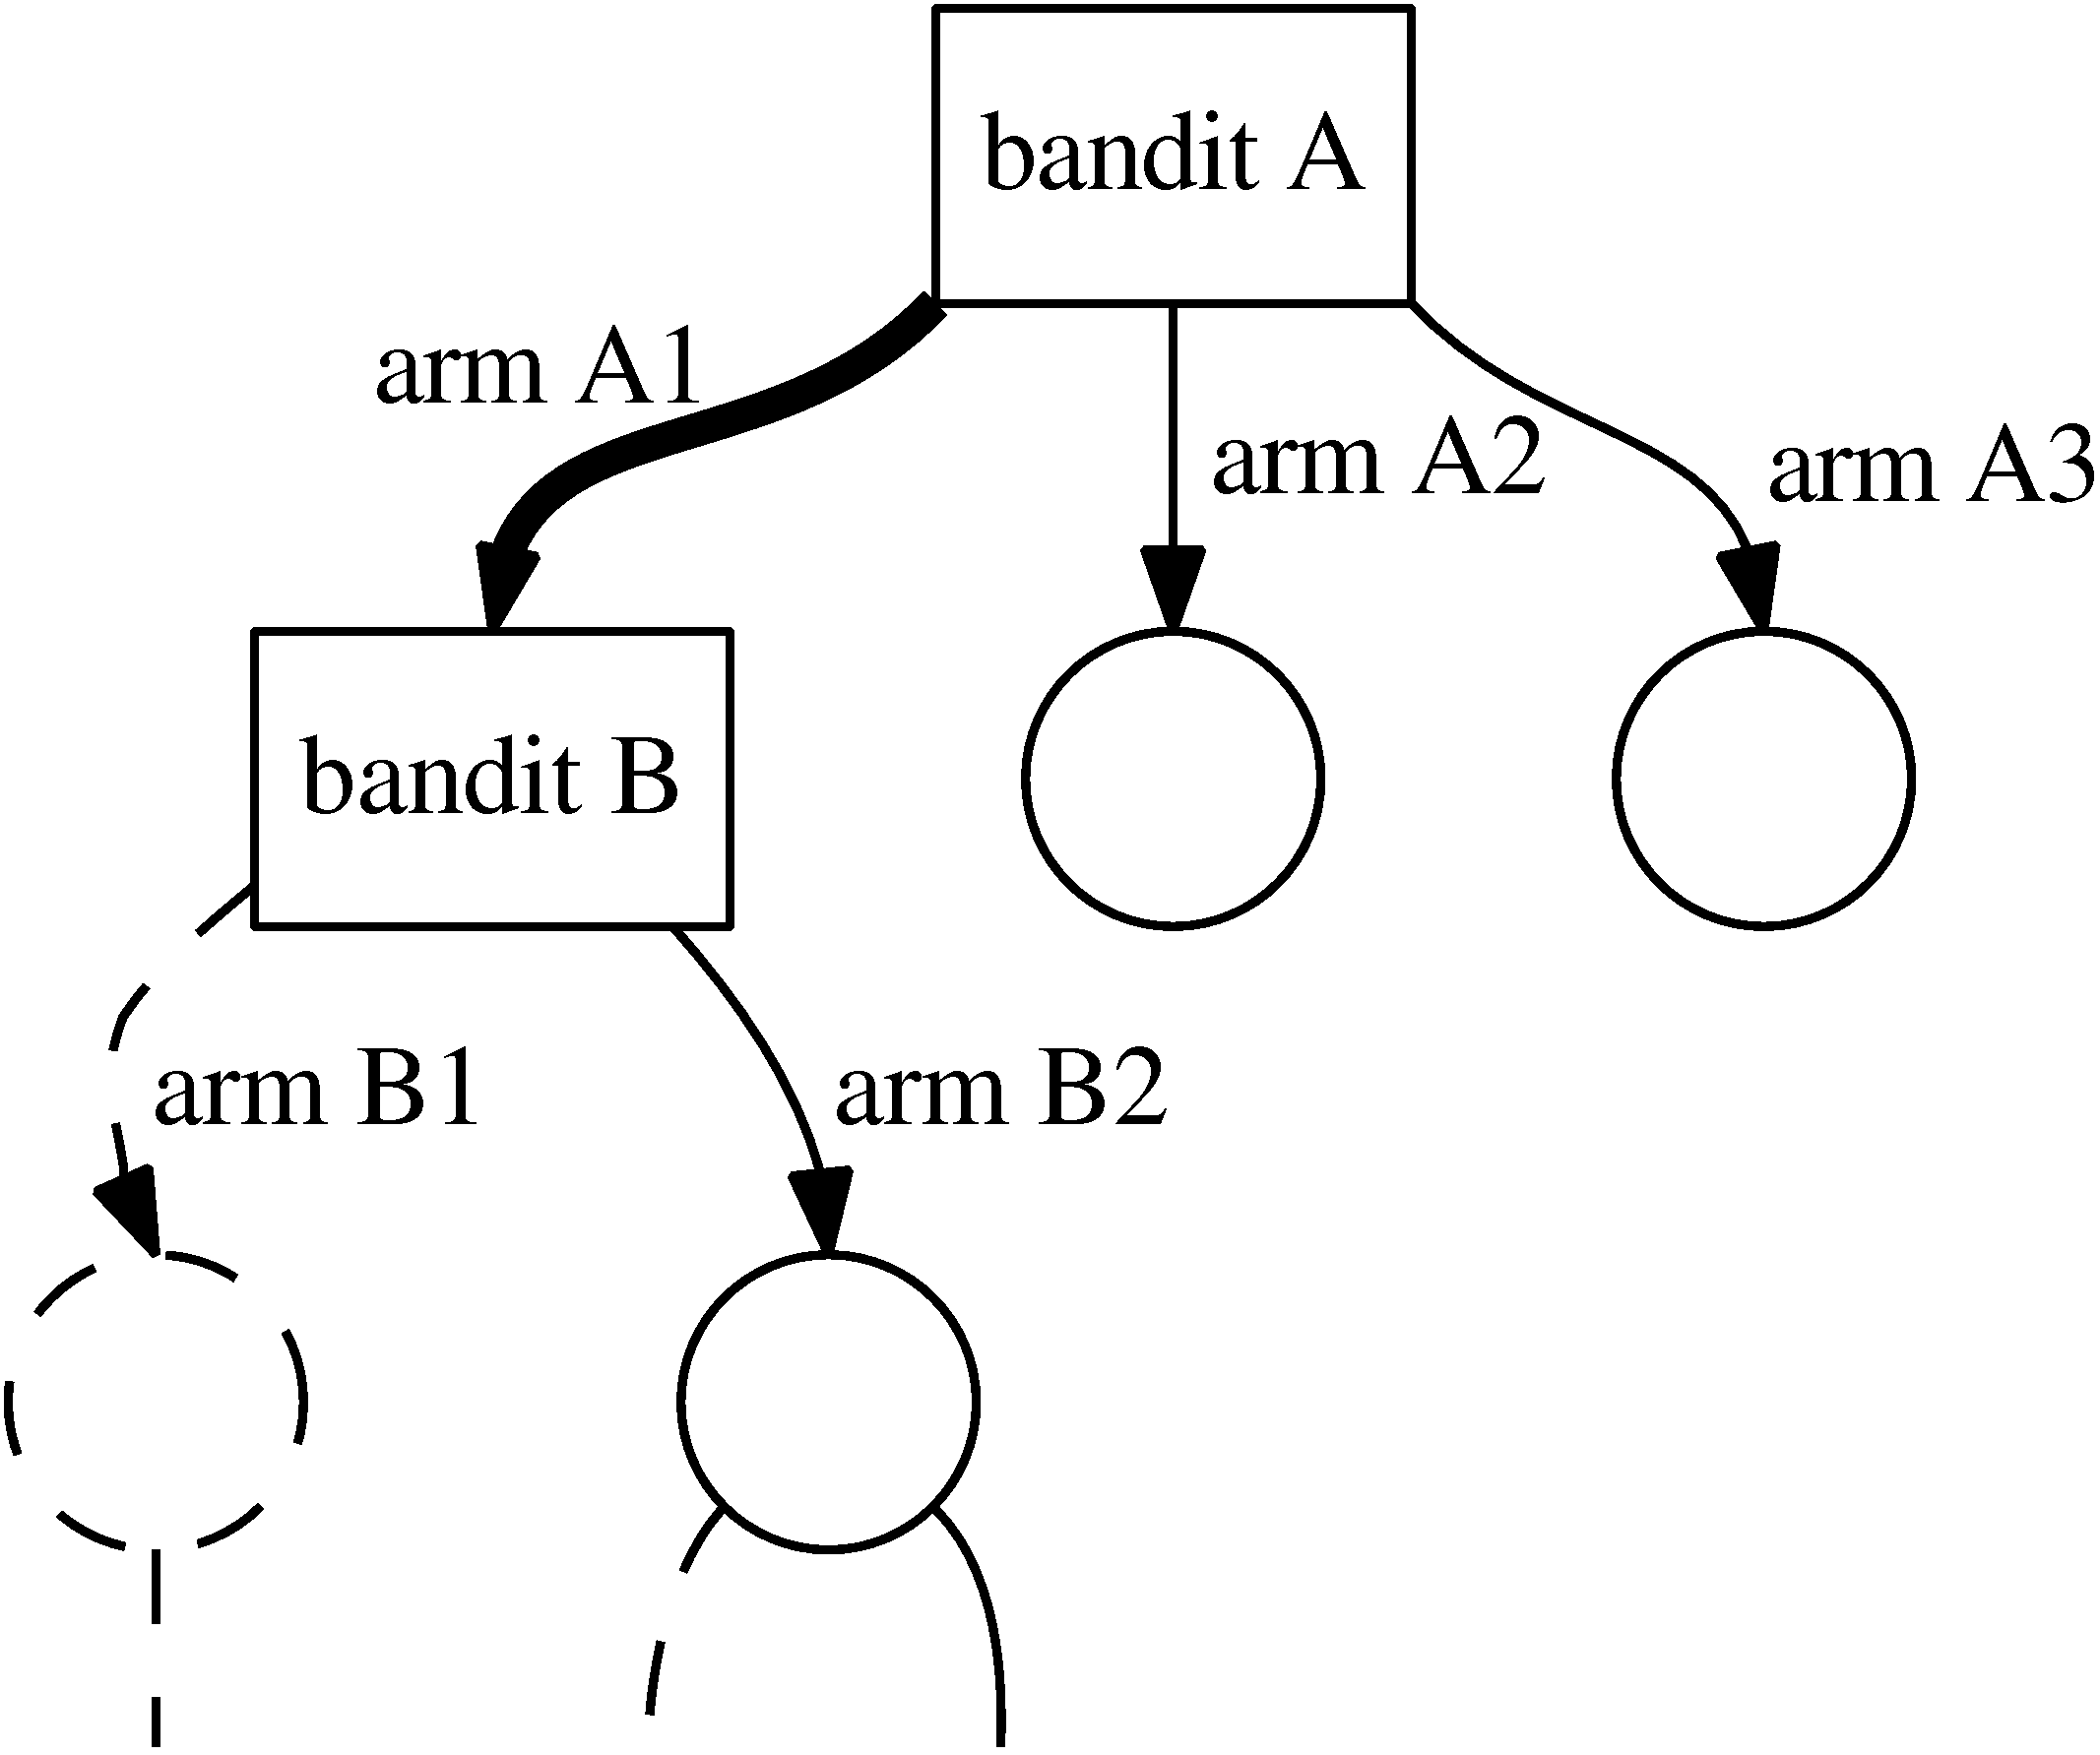
\includegraphics[scale=0.5]{figs/bandit_cascade.png}
    \end{center}


\end{frame}

\begin{frame}
    \frametitle{UCB en pratique}
    \begin{itemize}
        \item Ajout d'un paramètre $p$ de contrôle de l'exploration:
            $$ \hat{\mu}_{i,t-1} + {\color{blue}p} \sqrt{\frac{\log(t)}{T_i(t-1)}} $$
        \item Ajout de connaissances a priori $C_i(t)$:
            $$ \hat{\mu}_{i,t-1} + p \sqrt{\frac{\log(t)}{T_i(t-1)}} + {\color{blue} C_i(t)} $$
    \end{itemize}
    
\end{frame}

\begin{frame}
    \frametitle{Améliorations}
    \begin{itemize}
        \item Réduire le nombre de bras du bandit
        \item Ajout de connaissances expertes 
        \item AMAF
        \item ...
    \end{itemize}
    
\end{frame}



\frame{
  \frametitle{Echelle de niveau}

  TODO
}

\frame{
  \frametitle{Première victoire en 9x9}

  TODO
}

\section{Conclusion}

\frame{
  \frametitle{Alphago}

  TODO principe en 1 slide
}

\frame{
  \frametitle{Echelle de niveau}

  TODO
}

\frame{
  \frametitle{Autres applications}

  TODO
}

\frame{
  \frametitle{Conclusion}

  TODO
}

\frame{
  \frametitle{References}
  TODO

}





%\frame{
%  \frametitle{Exemple borne}
%
%\centering
%
%\begin{tikzpicture}
%
%    \node [circle,draw] (a) at (0,0) {a};
%    \node [circle,draw] (b) at (3,0) {b};
%    \node [circle,draw] (c) at (6,0) {c};
%    \node [circle,draw] (d) at (0,-4) {d};
%    \node [circle,draw] (e) at (-3,-4) {e};
%
%    \draw [dashed] (a) -- (b) node [pos=0.5]{\textbf{3}};
%    \draw [dashed] (a) -- (d) node [pos=0.3]{\textbf{4}};
%    \draw [dashed] (a) -- (e) node [pos=0.5]{\textbf{5}};
%  
%    \draw [dashed] (b) -- (c) node [pos=0.5]{\textbf{3}};
%    \draw [dashed] (b) -- (d) node [pos=0.3]{5};
%    \draw [dashed] (b) -- (e) node [pos=0.3]{7};
%  
%    \draw [dashed] (c) -- (d) node [pos=0.5]{\textbf{7}};
%    \draw [dashed] (c) -- (e) node [pos=0.3]{10};
%  
%    \draw [dashed] (d) -- (e) node [pos=0.5]{\textbf{3}};
%\end{tikzpicture}
%
%    \begin{block}{Calcul de la borne}
%        trajet déjà effectué = $\emptyset$
%
%        $(\underbrace{3+4}_{a}+\underbrace{3+3}_{b}+\underbrace{3+7}_{c}+\underbrace{3+4}_{d}+\underbrace{3+5}_{e})/2=19$
%    \end{block}
%
%}


\end{document}
